\begin{opin}{\guscolor}{Gustavo}

\subsubsection{Recursos educativos en el aula}
Durante la clase de hoy, Raquel nos hizo ver la gran cantidad de recursos didácticos existentes hoy en día en el mundo de las matemáticas. Veo una ventaja muy evidente respecto a buscarlo por nuestra cuenta y es que sin duda Raquel, como docente con años de experiencia, nos ha filtrado los recursos para evitar perdernos en la red.

Esto nos va a ayudar en nuestro futuro profesional como docentes ya que será un espacio dónde poder apoyarnos. Entre otro de los consejos que nos dio Raquel está el de que tenemos que asumir que es difícil estar al día de todo por lo tanto no hay que abrumarse por tal situación.

Los recursos a destacar son:

\subsubsection{Recursos del INTEF}
El Instituto Nacional de Tecnologías Educativas y de Formación  (INTEF) del Profesorado es la unidad del Ministerio de Educación, Cultura y Deporte responsable de la integración de las TIC en las etapas educativas no universitarias. Tiene rango de Subdirección General integrada en la Dirección General de Evaluación y Cooperación Territorial que, a su vez, forma parte de la Secretaría de Estado de Educación, Formación Profesional y Universidades (Fuente: \url{http://educalab.es/intef/introduccion})

Los siguientes recursos se encuentran disponibles desde la web del INTEF \url{http://educalab.es/recursos}, aunque también son interesantes los recursos específicos de matemáticas encontrados en el histórico de recursos \url{http://educalab.es/web/web/recursos/historico/asignaturas/matematicas}

\paragraph{Procomún}
\url{https://procomun.educalab.es/}

PROCOMÚN es el espacio que más destaca dentro de los recursos del INTEF y se describe como una red de Recursos Educativos Abiertos. Este espacio destaca por la gran cantidad de recursos disponibles y por la posibilidad de búsqueda de dichos recursos por medio de los metadatos.

Dentro de Procomún se hizo mención al Proyecto Gauss.

\paragraph{eXeLearning}
\url{http://exelearning.net/}

eXeLearning es una herramienta de autor de código abierto para ayudar a los docentes en la creación y publicación de contenidos web. Facilita la creación de contenidos educativos sin necesidad de ser experto en HTML o XML. Se trata de una aplicación multiplataforma que nos permite la utilización de árboles de contenido, elementos multimedia, actividades interactivas de autoevaluación… facilitando la exportación del contenido generado a múltiples formatos: HTML, SCORM, IMS, etc.

Características destacadas de Exelearning:
\begin{itemize}
\item Permite crear un árbol de navegación básico que facilitará la navegación.  

\item Permite escribir texto y copiarlo desde otras aplicaciones.  

\item Permite incluir imágenes, pero no es un editor de imágenes como Photoshop o Gimp.  

\item Permite incluir sonidos, pero deben estar grabados previamente con otra aplicación.  

\item Permite incluir vídeos y animaciones, pero no permite crearlas.  

\item Permite incluir actividades sencillas: preguntas de tipo test, de verdadero/falso, de espacios en blanco...  

\item Permite embeber elementos multimedia como vídeos, presentaciones, textos o audios.  

\item Permite incluir actividades realizadas con otras aplicaciones 
\end{itemize}


\paragraph{Proyecto Gauss}
\url{http://recursostic.educacion.es/gauss/proc/}

El Proyecto Gauss ha sido desarrollado por el INTEF. Es un proyecto específico de matemáticas y ofrece a los profesores varios centenares de ítems didácticos y de applets de GeoGebra, que cubren todos los contenidos de matemáticas de Primaria y de Secundaria.

\paragraph{Proyecto Agrega/Agrega2}
\url{http://www.agrega2.es/web/}

Este proyecto es una federación de repositorios de contenidos educativos digitales donde todo el mundo pueda buscar, visualizar y descargar material educativo digital no universitario.  Se pretende facilitar a la comunidad educativa una herramienta útil para integrar las Tecnologías de la Información y la Comunicación en el aula

Existe una segunda versión de este proyecto que mejora la anterior y se llama Agrega2. Es de los repositorios más complicados para encontrar cosas. De hecho, hay un curso específico para buscar contenidos en Agrega2.

\paragraph{Red de Buenas PracTICas 2.0}
\url{http://recursostic.educacion.es/buenaspracticas20/web/}

Red de Buenas Practicas 20 es una red social de profesores dentro del INTEF.

\paragraph{Internet en el aula}
\url{http://internetaula.ning.com/}

Otra red social para docentes

\paragraph{Educa con TIC}
\url{http://www.educacontic.es/recursos-educativos}

Es un blog especializado en el uso de las TIC en las aulas

\paragraph{Proyecto Descartes}
\url{http://proyectodescartes.org/}

El Proyecto Descartes comienza su andadura en el año 1998. Lleva mucho tiempo activo, por tanto es lógico pensar que hay mucha documentación y muchos recursos.

Hay una página antigua en una web oficial del ministerio (\url{http://recursostic.educacion.es/descartes/web/}) pero está sin mantenimiento. Esta página antigua lo tenían hecho en JAVA y daba tantos problemas a los usuarios que decidieron cambiarla. Aun así, todavía hay muchos recursos que redirigen de la nueva a la antigua.

La web actual del proyecto Descartes pertenece a la Red Educativa Digital Descartes, que explicamos a continuación.

\paragraph{Red Educativa Digital Descartes}
La Red Educativa Digital Descartes (RED Descartes) es una asociación no gubernamental que se ha constituido el 1 de junio de 2013. Los socios fundadores son profesoras y profesores que tienen una historia conjunta construida, durante quince años, desarrollando proyectos del Ministerio de Educación español, entre los que podemos citar el Proyecto Descartes, Educación Digital a Distancia, Proyecto Canals, Pizarra Interactiva, Newton, Experimentación Didáctica en el Aula, WikididácTICa y Buenas Practicas 2.0. (Fuente: \url{http://www.educacontic.es/blog/matematicas-interactivas-con-descartes-en-tablets-y-smartphones})

En la parte de arriba de la web hay un apartado de subproyectos que te lleva a la página web \url{http://proyectodescartes.org/indexweb.php} . Entre estos subproyectos destacan:
\begin{itemize}
\item Telesecundaria (\url{http://proyectodescartes.org/Telesecundaria/}): educación a través de videos. Ojeando esta aplicación, también hay ejercicios y explicaciones interactivas hechas con HTML5, lo cual hace que sea accesible a través de cualquier navegador moderno. 

Telesecundaria es además una modalidad en el sistema educativo de México.

 

\item Proyecto Canals (\url{http://proyectodescartes.org/canals/index.htm}) de la profesora catalana Maria Antònia Canals para infantil y primaria. 

 

\item Proyecto "EDAD" Educación Digital con Descartes (\url{http://proyectodescartes.org/EDAD/index.htm}) surge con el propósito de desarrollar recursos educativos digitales interactivos, para la Educación Secundaria Obligatoria (ESO) en las áreas curriculares de Matemáticas, Ciencias Naturales y Física y Química, que permitan su uso tanto en la enseñanza presencial como en la formación a distancia. 

 

\item Proyecto ASIPISA (\url{http://proyectodescartes.org/ASIPISA/index.htm}). ASIPISA es una palabra palíndroma, acrónimo de “Ayuda Sistemática Interactiva para PISA”, que da nombre a un proyecto de desarrollo de materiales educativos, digitales e interactivos, basados en las unidades liberadas del Programa internacional PISA 

 

\item Proyecto Competencias (\url{http://proyectodescartes.org/competencias/index.htm}): Pensado para formar en competencias como marcan los nuevos planes de estudios. Esta web recoge objetos de aprendizaje interactivos cuyo objetivo es la formación y evaluación competencial. Sus contenidos se basan en las unidades liberadas de PISA, en las de las Pruebas de Evaluación de Diagnóstico de diferentes Comunidades autónomas españolas de acuerdo a la Ley Orgánica de Educación (LOE) de 2006 y a las pruebas de Evaluación de diagnóstico establecidas por la Ley Orgánica para la Mejora de la Calidad Educativa (LOMCE) de 2013. 
\end{itemize}

\paragraph{Educarex}
Es el Portal con contenidos educativos de la Comunidad Extremadura. Extremadura estaba a la cola en educación e hizo un esfuerzo bestial para ponerse a la altura del resto de España. Este portal es parte del fruto de dichos esfuerzos.

\paragraph{Otros recursos}
Además de todo lo visto hasta ahora también existen otros recursos como revistas, blogs, páginas de internet, etc. A continuación se citan algunos de estos recursos para su conocimiento:
\begin{itemize}
\item Aulaplaneta es un sistema integrado de contenidos curriculares que pone al servicio del profesor una propuesta didáctica personalizable y gran variedad de recursos digitales para preparar sus clases, y a disposición de los alumnos todo lo que necesitan para aprender de forma motivadora y eficaz. Destacar el artículo ” Diez canales educativos imprescindibles de YouTube para alumnos y profesores” \url{http://www.aulaplaneta.com/2015/10/27/recursos-tic/diez-canales-educativos-imprescindibles-de-youtube-para-alumnos-y-profesores/}  

 

\item MisMates y TutorMates. Se trata de dos proyectos digitales de Oxford destinados para el área de Matemáticas.   

MisMates es una aplicación educativa de acceso exclusivamente on line y está enfocada al alumnado de entre 1º y 4º de la ESO que tiene a su disposición varias áreas de trabajo, un editor de expresiones matemáticas y una libreta digital.

TutorMates es una aplicación de escritorio para Windows, iOS o Linux, y trabaja con herramientas específicas los contenidos de cada bloque

 

\item Educacion 3.0 es una revista de elevado interés en el mundo educativo en el que destaca el artículo “15 recursos de Internet imprescindibles para cualquier profesor” \url{http://www.educaciontrespuntocero.com/recursos/recursos-para-educacion-profesor-imprescindibles/35931.html}  

 

\item ScolarTIC es un proyecto de la Fundación Telefónica. Es una Comunidad Educativa de ámbito hispano. Es un espacio social de aprendizaje, innovación y calidad educativa en el que se ofrecen cursos online gratis, recursos para el aula así como charlas, ponencias y talleres.  

 

\item Y además a nivel particular hay muchas webs de profesores que ponen su trabajo al servicio de los demás: 
\begin{itemize}
\item Pilarleku@ (\url{http://pilarlekunew.blogspot.com.es/}) 

\item Domingo Mendez \url{http://domingomendez.es/} y su blog “Educación y TIC” \url{http://domingomendez.blogspot.com.es/}  

\item Algebra con Papas \url{https://www.edu.xunta.es/espazoAbalar/sites/espazoAbalar/files/datos/1291360755/contido/index.htm}  

\item Thatquiz \url{https://www.thatquiz.org/es/} Web con cuestionarios de matemáticas 

\item Manuel Sada Allo y su web Ejemplos diversos de webs interactivas de Matemáticas \url{http://docentes.educacion.navarra.es/msadaall/geogebra/}  

\item Sectormatematica \url{http://www.sectormatematica.cl/}  

\item Antonio Perez Sanz \url{http://platea.pntic.mec.es/}~aperez4/. Antonio presentó los programas de TVE de “Más por menos” y “Universo Matemático”. Actualmente (Diciembre de 2016) es responsable de divulgamat. 

\item “Amo las mates” actualmente en la web \url{https://www.matematicasonline.es/}  

\item Disfruta las matemáticas \url{http://www.disfrutalasmatematicas.com/}  

\item Vitutor \url{http://www.vitutor.com/} también se usa para la universidad. Tiene un contenido de bachillerato bastante potente. es una plataforma de teleformación diseñada para el aprendizaje en línea de distintas materias. 

El proyecto comenzó con la especialización en contenidos de Matemáticas, y estamos trabajando en otras materias, como inglés.

\item  “Aula21” que en su página \url{http://www.aula21.net/primera/matematicas.htm}  recopila un listado de enlaces a recursos de interés en el mundo de las matemáticas. 

\item Banco de recursos de SM \url{http://www.smconectados.com/Banco_de_recursos.html} donde encontrarás recursos para ayudarte a hacer más fácil tu trabajo en el aula. 
\end{itemize}
\end{itemize}

\paragraph{9 cosas que los profesores digitalmente competentes hacen habitualmente}


\vspace{2cm}
\end{leftbar}
\vspace{-2cm}
\begin{figure}[hbt]
	\begin{leftbar}{\guscolor}
		\centering
		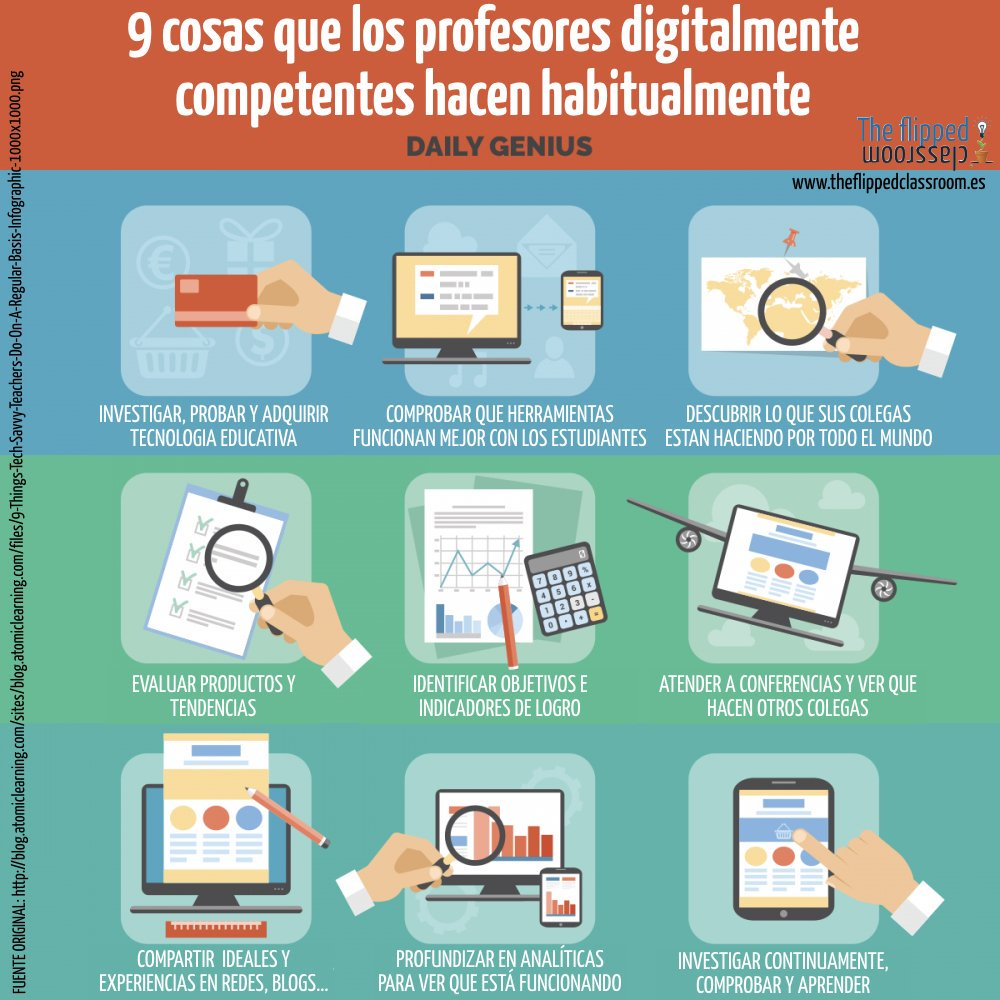
\includegraphics[width=0.8\linewidth]{img/9cosasdegus.jpg}
		\caption{9 cosas que los profesores digitalmente competentes hacen habitualmente.}
	\vspace{2cm}
	\end{leftbar}
\vspace{-2cm}
\end{figure}

\begin{leftbar}{\guscolor}
\vspace{-1.8cm} 
\paragraph{Uso del video en educación}
No cabe duda que el uso del video en la clase es una metodología innovadora. Está claro que tiene muchas ventajas como por ejemplo la de romper con la monotonía de la clase, pero también puede haber inconvenientes.

Los tipos de videos educativos según \url{http://www.uclm.es/profesorado/ricardo/Video/2002_2003/sld003.htm} son:

\begin{itemize}
\item \textbf{Documentales:} muestran de manera ordenada información sobre un tema concreto. 

\item \textbf{Narrativos:} tienen una trama narrativa a través de la cual se van presentando las informaciones relevantes para los estudiantes.  

\item \textbf{Lección monoconceptual:} son vídeos de muy corta duración que se centran en presentar un concepto.  

\item \textbf{Lección temática:} son los clásicos vídeos didácticos que van presentando de manera sistemática y con una profundidad adecuada a los destinatarios los distintos apartados de un tema concreto .  

\item \textbf{Vídeos motivadores:} pretenden ante todo impactar, motivar, interesar a los espectadores, aunque para ello tengan que sacrificar la presentación sistemática de los contenidos y un cierto grado de rigor científico. 
\end{itemize}

Un video motivador para poner a los alumnos puede ser el video de Tadeo Jones \url{http://www.telecinco.es/tadeojones/descubre-con-tadeo/Tadeo_Jones-Descubre_con_Tadeo-Matematicas_2_1697355179.html}

Otro video que impresiona a la hora de demostrar como la perspectiva puede engañar a como nuestro ojo le pasa la información a nuestro cerebro es \url{https://www.youtube.com/watch?v=U9PZizBDBZw} en el que colocando una serie de velas en un suelo plano y la posición de la cámara el autor nos muestra como da la sensación de que se acaba formando un cubo en 3 dimensiones sobre el que es capaz de sentarse.

Otro video fascinante es el de las potencias de 10 \url{https://www.youtube.com/watch?v=fbCwkfrKuaw} en el que nos muestran un “zoom out” con 10 elevado a n veces para salir al espacio y un “zoom in” con $\rfrac{1}{10}^n$ para adentrarnos en el organismo de las personas. El zoom out es otra manera de explicar los Sistemas de Información Geográfica como puede ser el de Google Maps.

Recursos de videos educativos pueden ser:
\begin{itemize}
\item El canal derivando de Youtube que son videos de Eduardo Sáenz de Cabezón \url{https://www.youtube.com/channel/UCH-Z8ya93m7_RD02WsCSZYA} 

\item “La pizarra de Fonemato” (www.matematicasbachiller.com) que contiene videos explicativos con una característica muy peculiar y es que lo explica todo muy despacio con un tono de voz serio que a la vez puede resultar cómico. 

\item El portal MatematicasIES \url{http://matematicasies.com} creado por Daniel López Avellaneda, Licenciado en Ciencias Matemáticas por la Universidad de Granada y Profesor de Matemáticas y Coordinador TIC en el IES Mar Serena. 

\item El portal Educacion 3.0 visto anterormente tiene recursos para crear videos como profesores. \url{http://www.educaciontrespuntocero.com/experiencias/recursos-para-grabar-lecciones-en-video/33017.html}  

\item Unicoos que es un portal de videos gratuitos para las asignaturas de ciencias. Enfocado a estudiantes de Secundaria, Bachillerato y universitarios.  

El portal Unicoos de YouTube proporciona algo más de 600 vídeos gratuitos para las asignaturas de Matemáticas, Física y Química. \url{https://www.youtube.com/user/davidcpv}
\end{itemize}

\paragraph{Matemáticas recreativas}
“La matemática recreativa se concentra en la obtención de resultados con actividades lúdicas, y a difundir o divulgar de manera entretenida y divertida los conocimientos o ideas o problemas matemáticos. Es un concepto tan viejo como lo son los juegos en los que interviene la lógica o de algún modo el cálculo” (Fuente: Wikipedia)

Es importante que los alumnos lleguen a ver que todos los juegos tienen una explicación matemática detrás. Llegar a sorprenderles es algo que logra captar su atención. Si recordamos en la página www.divulgamat.net hay una sección llamada Sorpresas Matemáticas en la que podremos encontrar bajo el menú principal recursos de este tipo


 
Un video que \textbf{llega a sorprender} a los alumnos es el de “crear chocolate de la nada” \url{https://www.youtube.com/watch?v=Y13tSEyOqGs.} En el video se consigue partir el chocolate y luego volver a reconstruir dando la sensación de que sobra una onza de chocolate. En realidad no se crea chocolate, es un truco creado que trabaja con diferentes pendientes de la recta que son cercanas y se puede manipular para aparentar que vuelve a su estado natural cuando no es cierto. La explicación detallada está en este otro video \url{https://www.youtube.com/watch?v=eb2hCmc2xso}

 

\paragraph{Anamorfismo y futbol\\}
 

\begin{minipage}[h]{1\linewidth}
	\centering
	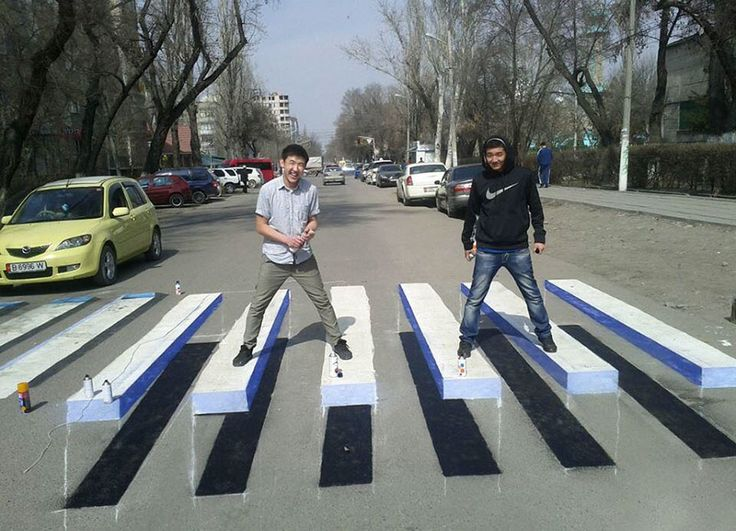
\includegraphics[width=0.7\linewidth]{img/anamorf1.jpg}
\end{minipage}
 
Otro ejemplo de matemáticas recreativas es el del anamorfismo. Consiste en deformar la imagen a través de efectos ópticos o a través de un procedimiento matemático con perspectivas. Uno de los artistas más destacados utilizando esta técnica es Julian Beever. “Julian es un artista británico que se dedica a dibujar con tiza. Ha creado dibujos de tiza en 3D en el pavimento utilizando un método llamado anamorfosis que crea una ilusión óptica. Sus dibujos en las calles desafían las leyes de la perspectiva. Ha logrado una técnica que le da un gran realismo a la imagen” (Fuente: Wikipedia).

\begin{minipage}[h]{1\linewidth}
	\centering
	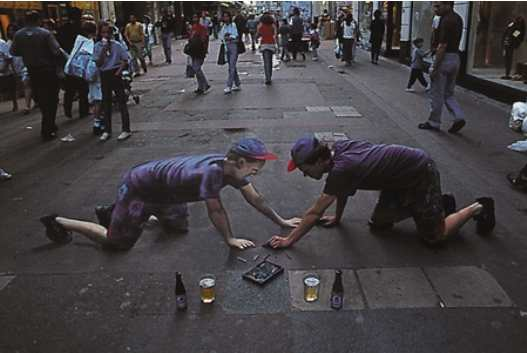
\includegraphics[width=0.7\linewidth]{img/anamorf2.jpg}
	
\end{minipage}
 
Un ejemplo de anaformismo de un cubo de Rubik en video se puede ver en  \url{https://www.youtube.com/watch?v=ooY7Mf0JlNM.} En este video nos permiten incluso acceder a la imagen que permite hace dicho anaformismo. Se puede descargar de \url{https://docs.google.com/file/d/0B3gyYFZJgwKVZ24zWDV1VVB5Wms/edit.} De hecho, me he descargado la imagen.

\begin{minipage}[h]{1\linewidth}
	\centering
	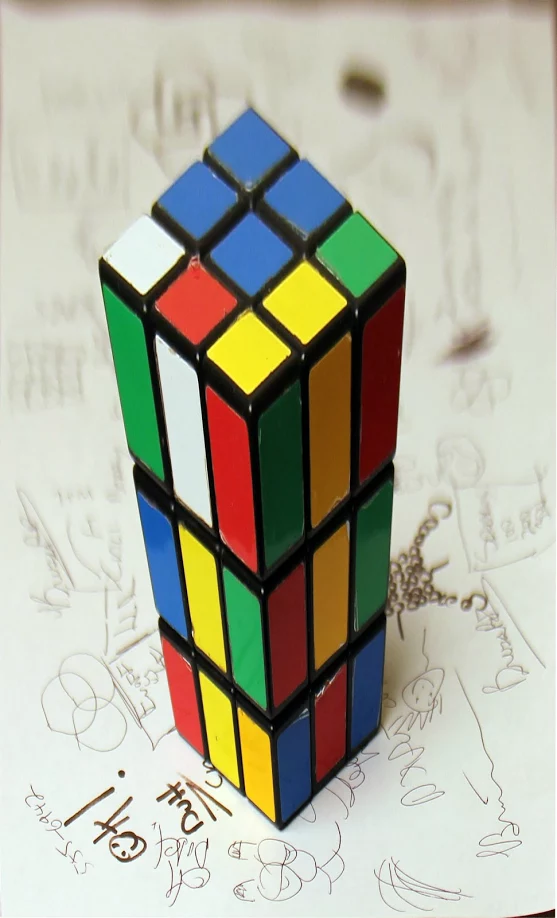
\includegraphics[width=0.45\linewidth]{img/anamorf3.png}
\end{minipage}
 
Por último, nos preguntaremos que tiene que ver el futbol con el anamorfismo. Pues bien, una vez visto que a la técnica que permite crear esta ilusión óptica se le llama anamorfismo, decir que en el futbol, principalmente en los partidos de primera división aprovechando el angulo de proyección de la grabación de las cámaras de televisión “colocan” la publicidad pintada en el plano para producir un efecto en 3D.

\begin{minipage}[h]{1\linewidth}
	\centering
	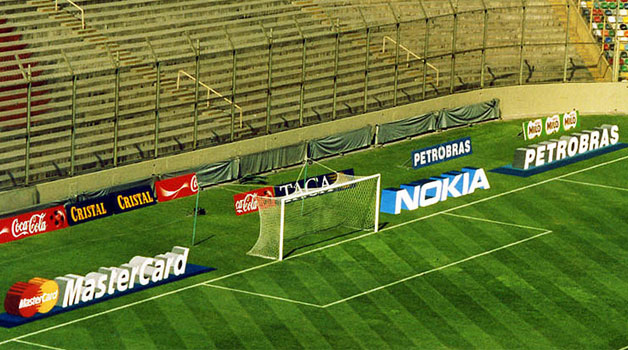
\includegraphics[width=0.7\linewidth]{img/anamorf4.jpg}
\end{minipage}
 
\paragraph{El cine y la literatura como recursos didacticos}
Por último, hay una gran cantidad de literatura matemática. No por ser matemáticos debemos olvidar la literatura. De hecho la convivencia entre ambas es fundamental.

Los siguientes enlaces tienen un montón de recursos literarios matemáticos:
\begin{itemize}
\item \url{http://aulamatematica.com/libros/libros_recomendados.htm}  

\item \url{http://www.librosmaravillosos.com/} en el que hay un buscador de libros gratuitos de difusión científica. 
\end{itemize}
El cine también ha servido como fuente de inspiración para muchos directores y guionistas a la hora de difundir las matemáticas:
\begin{itemize}
\item Una mente maravillosa 

\item El código Da Vinci 

\item Black Jack 

\item La vida es bella 

\item Cube 

\item Agora 

\item Contact 

\item Blade Runner 

\item El día de la bestia 

\item Moebius 

\item 3:19 

\item Granujas de medio pelo 
\end{itemize}
O como el caso de la “Jungla de Cristal 2” donde los protagonistas tienen que resolver el problema de las garrafas de 3 y 5 galones de agua. Para desactivar la bomba tienen que conseguir 4 galones exactos en una de las garrafas. ¿Cómo lo conseguirán? Aunque en la película no se explica claramente, se consigue (Fuente: \url{http://www.sociedadmatematicacantabria.es/Probl_Olimpiada/Sol_probl_3_2.htm}):
\begin{itemize}
\item 1º Llenas la de 5 y echas lo que puedas en la de tres.  

Quedan 3L en la de 3 y 2L en la de 5

\item 2º Vacías la de 3 y echas los 2L de la de 5 en la de 3.  

Quedan: 2L en la de 3 y 0L en la de 5

\item 3º LLenas la de 5 y echas lo que puedas en la de tres (1L)  

Quedan: 3L en la de 3 y 4L en la de 5

\item 4º Vacías la de 3 y ya tienes 4L en la de 5 
\end{itemize}

\paragraph{Khan Academy \url{https://es.khanacademy.org}}
Por último, no quería dejar sin mencionar en el portafolios la aportación realizada en el foro  por mi compañero de grupo Victor De Juan sobre la “Khan Academy”.

Khan Academy es una web que ofrece ejercicios de práctica, videos instructivos y un panel de aprendizaje personalizado que permite a los alumnos aprender a su propio ritmo, dentro y fuera del salón de clases. Y todo ello sin pagar ni un duro.

En este video de la Universidad Politécnica de Valencia nos explican cómo comenzar a usar esta web tanto si somos alumnos, profesores o padres. \url{https://www.youtube.com/watch?v=FvacPlqEw6g}

\end{opin}

\begin{opin}{\victorcolor}{Víctor}

Hoy ha sido un bombardeo de recursos para utilizar en clase. Paginas web, blogs, educalab... 
%
A día de hoy se me queda lejano porque no he profundizado sobre los recursos, porque creo que pueden caer en saco roto.
%
Parece que voy a tener que estudiarme y bucear por todos estos recursos para descubrir cuáles me gustan más, cuáles me parecen más útiles, etc.
%
Y este trabajo tendrá pleno sentido cuando tenga delante un verano en el que prepararme las clases del año siguiente y busque, más concretamente, como tratar algún contenido o me quiera apoyar en alguno de estos recursos para un tema específico que el año anterior no funcionó en clase la manera en la que lo hice.

Son tantísimos recursos que ahora no he podido profundizar en ellos, pero que me los he descargado todos para poder trabajar sobre ellos más adelante.

\subsubsection{Gamificación}

Este es un tema que no hemos llegado a ver en clase, pero sí en la charla de Javier de las jornadas complementarias.
%
Partiendo de la base de que \textit{La gamificación es como el ketchup. Hay veces que es genial, pero no soluciona absolutamente todos los problemas.} (Javier Espinosa), es un recurso muy muy interesante que, por como soy, creo que me encatará aplicar en el aula.
%
Tanto es así, que he elegido mi TFM a raíz de esto, para ser un docente gamificador. 
%
Creo que tengo mucho potencial en esta línea y espero aprender mucho con mi TFM.

\end{opin}

\begin{opin}{\pedrocolor}{Pedro}

Se presentan durante la clase varios recursos educativos, que permiten una mejor transmisión de conocimientos profesor-alumno. Cabe destacar la labor educativa del \index{INTEF} \textbf{INTEF (Instituto Nacional de Tecnologías Educativas y de Formación del Profesorado)}, encargado de la introducción de las TIC en las etapas educativas no universitarias. Destaca por:

\begin{itemize}

\item Su gran variedad de material de apoyo al profesorado, destinado a la continua actualización científica y didáctica del profesorado.
\item Elaboración y difusión de materiales en soporte digital y audiovisual, que permita hacer de las TICs un instrumento de trabajo cotidiano para el profesorado.
\item Mantenimiento del Portal de recursos educativos del Departamento y por la  creación de redes sociales que permita el intercambio de experiencias y recursos entre el profesorado.
\end{itemize}
Importante tener en cuenta que la web de INTEF ha sido sustituida por \url{http://educalab.es/home} dentro de la cual encontramos todos los recursos que pasamos a enumerar.


\begin{itemize}

\item \textbf{ Procomún:} Red de recursos educativos que permite compartir ideas y experiencias. Todos estos REAs están estructurados por niveles y materias. La variedad de recursos es múltiple y variada, desde fotografías, videos, problemas, ilustración, etc. Podemos participar en comunidades, redes sociales educativas, etc. 

\begin{minipage}[hbtp]{1.0\linewidth}
\centering
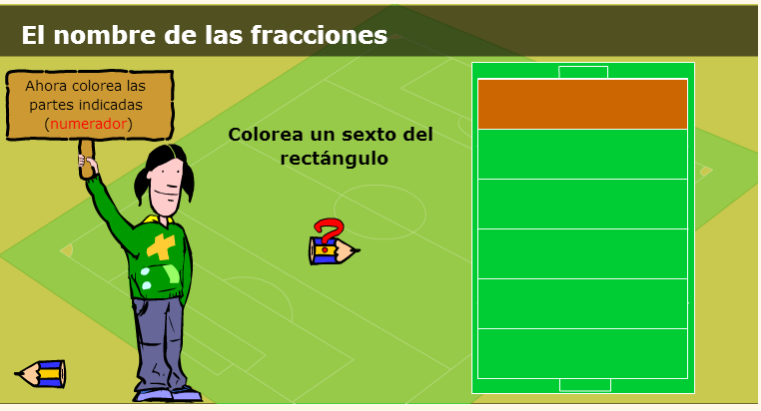
\includegraphics[scale=0.36]{img/intefpedro1.png}
%\captionof{figure}{...}
\end{minipage}

 
\item \textbf{ eXeLearning:} Considero que es una herramienta útil. Me permite, sin tener grandes conocimientos sobre lenguajes de programación, crear actividades de verdadero-falso, ejercicios de elección múltiple, actividades desplegables de relleno de huecos, etc. 
%
En la figura \ref{fig:exelearningPedro} encontramos un ejemplo.
\end{itemize}

\vspace{2cm}
\end{leftbar}
\vspace{-2cm}
\begin{figure}[hbtp]
\begin{leftbar}{\pedrocolor}
\centering
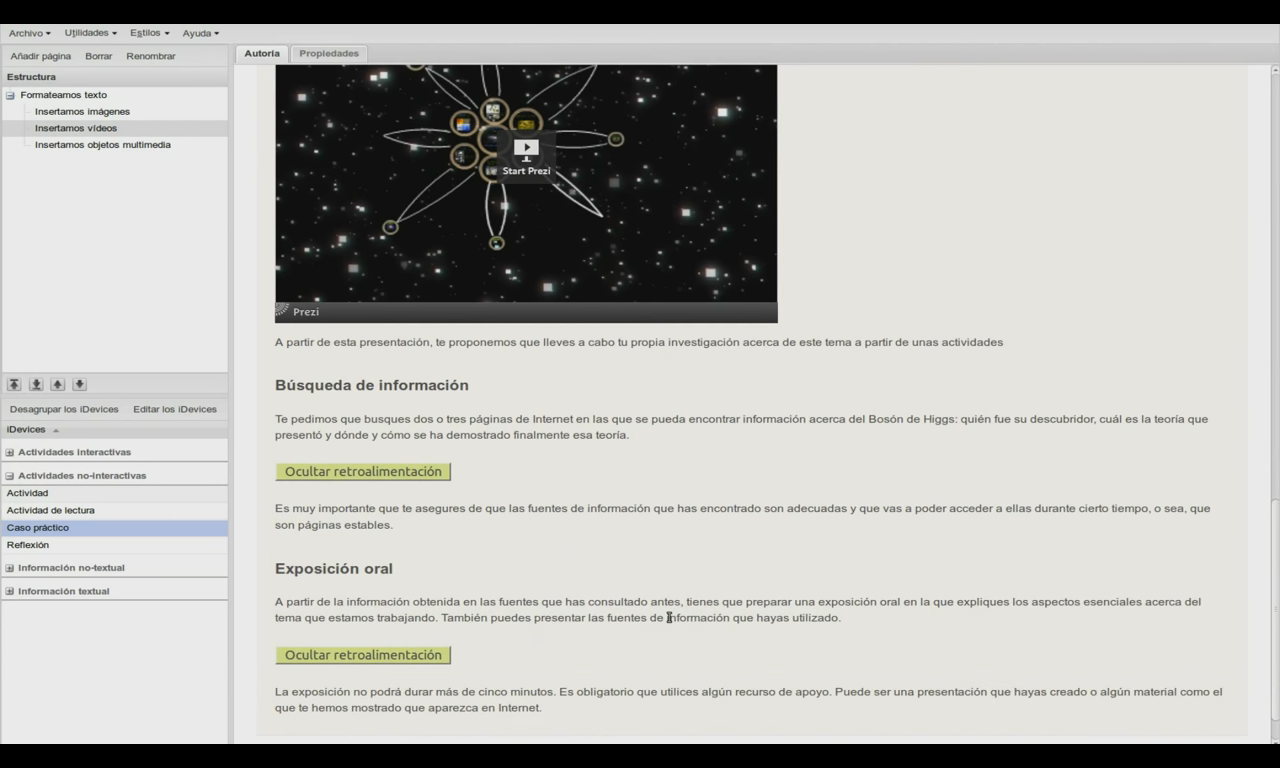
\includegraphics[scale=0.24]{img/intefpedro2.png}
\caption{Ejemplo de eXeLearning.}
\label{fig:exelearningPedro}
\vspace{2cm}
\end{leftbar}
\vspace{-2cm}
\end{figure}

\begin{leftbar}{\pedrocolor}
En el apartado de Documentación de \url{http://exelearning.net/category/documentacion/} encontramos desde el manual, hasta la versión portable del software.

\begin{itemize}


\item \textbf{Histórico de recursos:}  Permite el acceso a una gran cantidad de recursos educativos para la comunidad docente. Todos ellos ordenados por cursos, materias y unidades.  

\item \textbf{Proyecto Gauss:} Dentro de mis expectativas educativas, considero que es el recurso más interesante por centrarse en la asignatura de matemáticas. Brinda al profesorado varios centenares de ítems didácticos y de applets de GeoGebra (se pueden insertar en Geogebra), que cubren todos los contenidos de matemáticas de Primaria y de Secundaria. 

\item \textbf{EDA (Experiencia Didáctica en el Aula):} Proyecto que pretende mostrar al profesorado las ventajas e inconvenientes de utilizar estas nuevas tecnologías en el aula. 

\item \textbf{Agrega:} Repositorio de contenidos educativos. Su principal problema es la dificultad de buscar contenidos. Este buscador ha encontrado sustituto en Agrega2, permitiendo buscar unidades didácticas completas, recursos desagregados para la construcción de nuevos recursos, etc. 

\item \textbf{Red de Buenas Prácticas 2.0:} Red social de profesores que pone en común sus intereses. Destacar, dentro de la pestaña Inicio -> Recursos Educativos. Nos habla desde cómo crear un blog hasta como formarte en didáctica de TIC. 

\item \textbf{Proyecto Descartes:} Herramienta de trabajo para aquellos profesores que desean crear lecciones interactivas en el formato de páginas Web. 

\begin{itemize}

\item \textbf{Web inicial del Ministerio} -> \url{http://recursostic.educacion.es/descartes/web/} se encuentra ya sin mantenimiento. 

\item \textbf{Web \url{proyectodescartes.org}} -> Pertenece a una organización no gubernamental. 
\end{itemize}
\end{itemize}
 
Otros recursos educativos que merecen mención por su contenido son: Educarex y Educación 3.0. Esta última muy recomendable por su propósito de contribuir al cambio metodológico en las aulas a través de las TIC y de las metodologías activas.

Pese a todas estas web que recogen un contenido abrumador de recursos, no hay que subestimar el uso de videos educativos en el aula. Lo importante es la selección de los mismos:

\begin{itemize}

\item Contenido adecuado a la edad. 
\item Vocabulario cuidado. 
\item Claridad de la idea que se quiere transmitir. 
\item Duración media, que no llegue a cansar al alumno. 
 
\end{itemize} 
 
 
 
 
A continuación enumero los audiovisuales que más me han llamado la atención:
 

\begin{itemize} 

\item \textbf{La cuna de Halicarnaso} de José Antonio Lucero. Es sobre Historia, pero considero que el formato podría aplicarse perfectamente a la asignatura de matemáticas. Llegué a él gracias a Chema Lázaro, en su jornada de Flipped Classroom (Clase invertida). 
\item \textbf{Divermates }
\item \textbf{Descubre con Tadeo }
\item \textbf{Blog Mateomolivares} \url{http://matemolivares.blogia.com/}
\item \textbf{Fonemato} Videos de matemáticas de forma amena. Me aporta gran utilidad a la hora de ver como se podría impartir una clase, desde conceptos hasta la didáctica utilizada. 
\end{itemize} 
 
El profesor tiene que ser capaz de utilizar todo este material de una manera óptima, para captar la atención del alumno. Debemos ser capaces de asombrar, ofrecer desafíos y permitir que sean capaces de buscar estrategias de resolución. Por lo tanto, se hace necesario  saber \textit{dónde se encuentra la información, seleccionar la oportuna y dar el uso adecuado a la misma}.


\end{opin}

\begin{opin}{\virgicolor}{Virginia}


\subsubsection{Recursos educativos}

En primer lugar me gustaría destacar la frase que recalca Raquel en el tema: la labor del profesor no es demostrar todo lo que sabe sino saber cómo transmitir esos conocimientos. De nada sirve un ser un genio en una materia si luego nadie es capaz de entender lo que dice. Afortunadamente, hoy en día los profesores tienen la suerte de contar con multitud de recursos educativos para facilitar esa transmisión de conocimientos.

Me pareció una gran idea lo de la escuela 2.0 por el hecho de facilitar el aprendizaje de los alumnos a través de una herramienta básica de la era digital como son los ordenadores. A través de internet tenemos acceso a información ilimitada que puede ser de gran utilidad para mejorar el aprendizaje. Sin embargo, debido a que la inversión era muy alta, la idea se abandonó. Creo que habría que reconsiderar en que se invierte en este país ya que buenas inversiones a corto plazo pueden dar grandes resultados a largo plazo. Como bien dice el lema, sin educación no hay ciencia y sin ciencia no ha sanidad lo que muestra lo indispensable que es la educación para la buena marcha de un país con lo cual habría que reconsiderar y plantearse cómo mejorar el actual sistema educativo.

Cuando Raquel empezó a mostrar la cantidad de páginas webs que había con recursos tecnológicos para realizar las clases de una forma diferente, me quede bastante impresionada. También me animo a sentir la forma de enseñar con otra perspectiva. Reconozco que me da un poco de respeto el convertirme en profesora y caer en la rutina de la típica clase magistral en la que la mitad de los alumnos no atienden y la otra mitad no comprenden lo que se les cuenta. Todos estos recursos me hacen ver la educación de una forma más divertida y motivadora.

En primer lugar hablar del INTEF, Instituto Nacional de Tecnologías Educativas y de Formación a través del cual se llega a multitud de páginas con recursos educativos. Entre ellas llegamos a la siguiente página web \url{http://educalab.es/recursos} donde vimos un montón de recursos como procomún o exelearning aunque de especial interés me parece el histórico de recursos donde puedes ver aquellos que te interesen según la asignatura a impartir. Desde luego hay muchos interesantes, entre ellos el de laboratorio básico de azar, probabilidad y combinatoria donde las aplicaciones interactivas hacen más fácil la compresión del temario.

Dos recursos más conocidos e igualmente fundamentales son el proyecto descartes y el proyecto Gauss:

\begin{itemize}

\item \url{http://proyectodescartes.org/descartescms/} 

\item \url{http://recursostic.educacion.es/gauss/proc/} 
\end{itemize}

Las herramientas que tienen ambos proyectos es inmensa, creo que es muy interesante para cualquier profesor porque básicamente cualquier tema que se imaginen lo pueden encontrar en sus páginas webs. Dentro del proyecto Descartes me quedo con el proyecto EDAD ya que además de las matemáticas, por mi formación me gustaría poder dar clase también de física y química y precisamente el proyecto EDAD desarrolla recursos educativos digitales interactivos, para la educación secundaria obligatoria en las áreas curriculares de Matemáticas, Ciencias Naturales y Física y Química. En cuanto a la página del proyecto Gauss me gustó entre otras la aplicación de “La escalera de bomberos” para calcular las propiedades de los ángulos y la del “Tamaño relativo” para comprobar la exactitud de lo que vemos.

Otra de las páginas que me gusto fue la de educación de la comunidad autónoma de Extremadura donde por ejemplo para bachillerato hay un recurso interesante para el tema de los números complejos: \url{http://conteni2.educarex.es/mats/120077/contenido/}

Navegando un poco por Internet en las páginas que vimos en clase además de muchas otras que he descubierto buscando recursos educativos, me he dado cuenta de lo importante de 4 palabras que comenta Raquel al final de este apartado: Buscar-Analizar-Escoger-Adaptar. Esto es, son muchísimos los recursos de los que disponemos y por ello es necesario buscar aquellos que más nos interesen, analizarlos detenidamente para ver cuál de ellos es más útil en función de los alumnos que tengamos y de la unidad didáctica donde se quieran aplicar esos recursos, para finalmente escoger uno de ellos y adaptarlo en función de las necesidades educativas.

En este contexto, quiero poner el link de un blog que habla sobre los recursos tecnológicos e indica que para que dichos recursos sirvan de algo es necesario modificar las prácticas, es decir, el uso de tecnologías en educación implica nuevos planteamientos:
\url{http://matematicaeninicial5.blogspot.com.es/2010/01/los-recursos-tecnologicos-que.html}

\subsubsection{Uso del vídeo en educación}
También vimos este día el uso del vídeo en la educación que sirve para romper la monotonía de la clase pero hay que seguir una serie de pautas importantes en la elección del mismo ya que una elección o uso inadecuado del video podría ser más perjudicial que beneficioso. De la siguiente página web he recogido una imagen que resumen las funciones educativas del vídeo:
\url{http://miuras.inf.um.es/~oele/objetos/funciones_del_vdeo_en_la_educacin.html}


\begin{minipage}[hbtp]{1.0\linewidth}
	\centering
	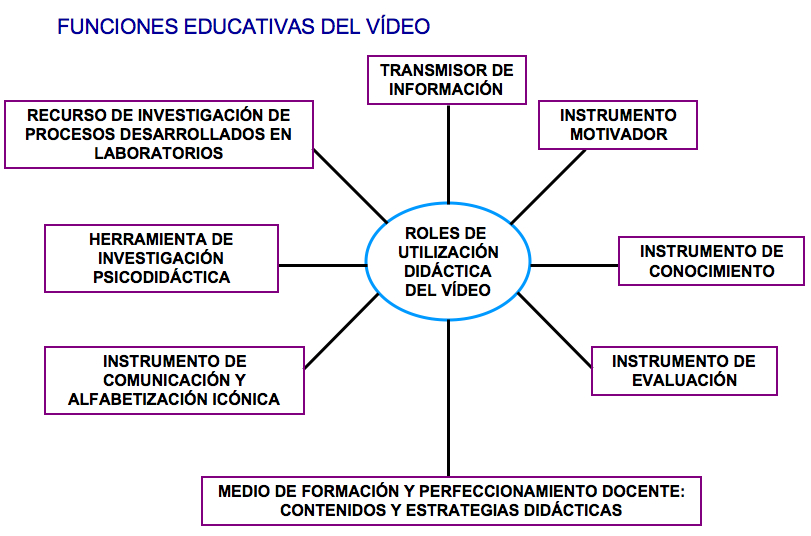
\includegraphics[width=0.85\linewidth]{img/videoeducacion.jpg}
	\captionof{figure}{Funciones educativas del vídeo}
	\label{videoeducacion}
\end{minipage}

demás, Salman Khan muestra la importancia del uso del vídeo para reinventar la educación: \url{https://www.ted.com/talks/salman_khan_let_s_use_video_to_reinvent_education?language=es}

Me pareció muy motivador el video de Tadeo Jones y bastante divertido la parodia del 3x2 de José Mota. Vimos diferentes páginas donde ver multitud de videos relacionados con las matemáticas. Anteriormente yo hablé de Eduardo Saénz de Cabezón porque vi videos suyos bastante interesantes y curiosamente en este punto Raquel nos presenta también videos suyos a través del Canal Derivando. En este canal me resultó muy curioso el vídeo sobre el espesor de una página de papel de 0.01 mm de grosor tras doblarla 54 veces:

\url{https://www.youtube.com/channel/UCH-Z8ya93m7_RD02WsCSZYA}

Buscando más videos de él encontré una presentación muy interesante de cerca de 1 hora en el que relaciona las matemáticas con los juegos, el viaje y el amor:

\url{https://www.youtube.com/watch?v=4zjQNPlOpaI}

Muy útiles y muchos recursos audiovisuales aparecen en las páginas de Fonemato y Únicoos entre otros. Este último especialmente interesante porque hay recursos también para física y química, lo que me está aportando muchas ideas a la hora de dar yo clase ya que física y química es también una de las asignaturas que me va a tocar dar durante mi periodo de prácticas además de las matemáticas.

\subsubsection{Matemáticas recreativas}

Las matemáticas recreativas utilizan actividades lúdicas para transmitir los conocimientos matemáticos de una forma diferente y más divertida. Hay multitud de recursos para aplicar esta matemática recreativa en el aula como son acertijos, cuentos, juegos, chistes, jeroglíficos, trucos de magia… Al final como ya se ha ido viendo a lo largo de la asignatura el objetivo es llegar al alumno de una forma diferente a la tradicional conectando el aprendizaje con las emociones, haciendo que les guste lo que aprendan y tengan una mayor motivación por seguir ampliando sus conocimientos.
A continuación indicó algunos de los recursos de los que vimos en clase:

\begin{itemize}

\item www.divulgamat.net: en especial el apartado de sorpresas matemáticas donde se incluyen entre otros acertijos, chistes… Un ejemplo de los que vi es el siguiente acertijo: 
El director de un instituto, el día que comenzó el curso 2002-2003, reunió a todos los alumnos en el estupendo salón de actos y les dijo:
\begin{enumerate}
\item En el instituto hay 250 alumnos y 250 casilleros.
\item En estos momentos están todos cerrados.
\item El alumno nº 1 abrirá todos.
\item El alumno nº 2 cerrará todos los casilleros pares.
\item El alumno nº 3 cambiará el estado de los casilleros 3,6,9,12,... Es decir, el que esté abierto lo cierra y el que esté cerrado lo abre.
\item El alumno nº 4 cambiará el estado de los casilleros 4,8,12,16,...
\item El alumno nº 5 cambiará el estado de los casilleros 5,10,15,20,...
\end{enumerate}
Y así sucesivamente hasta el alumno nº 250.
Después de este entretenido comienzo de curso, ¿cuantos casilleros quedarán abiertos?
\item \url{http://www.eduardoochoa.com/joomla/}: El saco del dinero que desmiente una típica cadena de whatsapp, el mítico de los 5 hijos… 

\item \url{http://matemolivares.blogia.com/temas/matematicas-y-humor.php.} En concreto la sección de matemáticas y humor, que mejor que aprender riendo. 

\item Anamorfosis matemática: aparte de los que vimos en clase quiero hablar de Jonty Hurwitz que aplica este concepto a la escultura (ver Figura \ref{anamorfisVir}: Anamorfosis matemática aplicada en la escultura (Jonty Hurwitz)).  \url{http://culturacolectiva.com/jonty-hurwitz-esculturas-matematicas/} 
\end{itemize}


\vspace{2cm}
\end{leftbar}
\vspace{-2cm}

\begin{figure}[hbtp]
	\begin{leftbar}{\virgicolor}
	\centering
	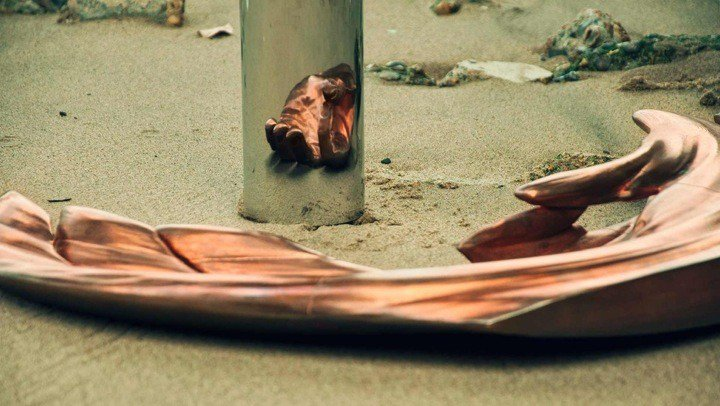
\includegraphics[width=0.6\linewidth]{img/viryin.jpg}
	\captionof{figure}{Anamorfosis matemática aplicada en la escultura (Jonty Hurwitz)}
	\label{anamorfisVir}

\vspace{2cm}
\end{leftbar}
\vspace{-2cm}

\end{figure}
\begin{leftbar}{\virgicolor}

\subsubsection{El cine y la literatura como recursos didacticos}
Por último, se habló del cine y la literatura relacionada con las matemáticas. Creo que tanto la lengua y literatura como las matemáticas son dos asignaturas imprescindibles por lo que hay que inculcar su importancia desde edades tempranas. Una buena forma de ver la utilidad de las matemáticas es leer libros interesantes que apliquen de una u otra forma algún tema matemático, así, además de crearles pasión por las matemáticas estamos además inculcando la importancia de la lectura (\url{http://www.aulamatematica.com/libros/libros_recomendados.htm}). Me parece un recurso vital que aporta grandes beneficios en el futuro del estudiante en dos de las principales asignaturas.

Por otro lado, como el cine es algo que suele gustar mucho a los jóvenes, que mejor forma de emocionarlos poniendo películas de moda que apliquen matemáticas de forma amena y divertida. Raquel nos puso el video de La jungla de cristal que recordaba gratamente ya que el día que la vi recuerdo de estar entusiasmada con mi familia realizando el acertijo para ver quien acertaba primero, y la motivación que me supuso acertarlo rápidamente.

Entre las películas con trasfondo matemático las que más me han gustado son: una mente maravillosa, El código Da Vinci, Black Jack y Agora.

\end{opin}
